\documentclass[12pt,twoside]{article}
\setcounter{tocdepth}{4}
\setcounter{secnumdepth}{4}

\usepackage[margin=0.7in]{geometry}

\usepackage{amsmath}
\usepackage{amsfonts}

\usepackage{fancyhdr}
\pagestyle{fancy}
\fancyhead{}
\fancyhead[RO,LE]{Causal Effects}
\fancyfoot{}
\fancyfoot[LE,RO]{\thepage}
\fancyfoot[LO,CE]{Section \thesection}

\usepackage{tikz}
\usetikzlibrary{positioning, calc, shapes.geometric, shapes, shapes.multipart, arrows.meta, arrows, decorations.markings, external, trees}

\tikzstyle{Arrow} = [
    thick,
    decoration={
        markings,
		mark=at position 1 with {
            \arrow[thick]{latex}
		}
	},
	shorten >= 3pt, preaction = {decorate}
]

\title{Identification and Estimation of Causal Effects}
\author{
    Lorenzo Fabbri
}


\begin{document}

\maketitle
\tableofcontents

\section{Resources}

\begin{itemize}
    \item Formulas for when there are more than two time points.
    \item G-computation, IPTW, and EIF-based estimators, including for multiple interventions.
    \item Do the terms $f(a|l)$ go away because we are setting the exposure $A$ to $a$, or are they incorporated with $f(l)$ into $f(a,l)$? If they are removed, where does the summation over $a$ come from for natural-value based interventions?
    \item What is the difference between $a^*$, $a$, and $a^{+g}$?
    \item E-mail Jessica SWIG; document fast food; GitHub discussion; StackExchange posts.
    \item $E[Y^g|l,a^{+g}]f(a^{+g}|a)$: what if $A$ is continuous? Just multiply?
\end{itemize}

%%%%%%%%%%%%%%%%%%%%%%%%%%%%%%%%%%
\section{Time-invariant Exposures}
%%%%%%%%%%%%%%%%%%%%%%%%%%%%%%%%%%

\subsection{Deterministic Treatment Regimes}
The rule for assigning treatment does so with probability 1.

\subsubsection{Deterministic Static Treatment Regimes}
The rule for assigning treatment does not depend on past treatment or covariates.

\begin{figure}[ht]
\centering
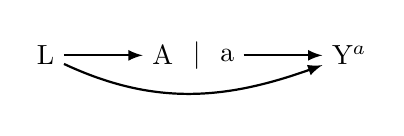
\begin{tikzpicture}[
array/.style={
    rectangle split,
	rectangle split parts = 3,
	rectangle split horizontal,
    minimum height = 2em
    }
]

\node (1) {L};
\node [array, right = of 1] (2) {
    {A}
    \nodepart{two}{$|$}
    \nodepart{three}{a}
};
\node [right = of 2] (3) {Y$^a$};

\draw[Arrow, thick] (1.east) -- (2.west);
\draw[Arrow, thick] (1) to [out=335, in=200] (3);

\draw[Arrow, thick] (2.east) -- (3.west);

\end{tikzpicture}
\caption{A SWIG representing a static treatment regime.}
\label{fig:swig_det_stat_inv}
\end{figure}

The joint density is:

\begin{equation}
    f(y,l,a) = f(y|l,a) f(a|l) f(l).
\end{equation}

After intervening on the exposure $A$, we have:

\begin{equation}
    f^G(y,l) = f(y|l,\textcolor{red}{a}) f(l).
\end{equation}

Thus, the expected value of the outcome $Y$ is:

\begin{align}
    \mathbb{E}^G \left[ Y \right] &= \sum_y y f^G(y) \\
    &= \sum_y y \sum_l f^G(y,l) \\
    &= \sum_y \sum_l y f(y|l,\textcolor{red}{a}) f(l) \\
    &= \sum_l \mathbb{E} \left[ Y|A=\textcolor{red}{a},L=l\right] f(L=l).
\end{align}

\paragraph*{Algorithms}
One estimator of $\mathbb{E}^G [Y]$ is called \textbf{parametric g-computation formula}, and is based on an outcome model alone. For the simple case of a deterministic static intervention with one exposure and a single time point, the pseudo-algorithm reads as follows:

\begin{enumerate}
    \item Fit a regression model with dependent variable $Y$ and independent variables $A$ and $L$.
    \item Estimate the outcome $Y^a$ using the model fit in the previous point but changing the exposure according to the intervention rule $G$.
    \item Take the average of $\hat{Y}^a$ over the confounders $L$.
\end{enumerate}

In the case of multiple exposures (e.g., if $A$ is actually a vector of variables), the g-formula would remain the same \footnote{We are assuming that there would be \textbf{no arrow} between exposure nodes in the SWIG, that is: $f(a_1,a_2|l) = f(a_1|l) \times f(a_2|l)$. This means that the correlation between them is due to e.g., a common source, but the exposures themselves are not causally related.}, but the pseudo-algorithm should be modified to take into account that the intervention rule now applies to all exposures $a \in \mathbf{A}$.

\subsubsection{Deterministic Dynamic Treatment Regimes}
The rule for assigning treatment depends on past treatment or covariates.

\begin{figure}[ht]
\centering
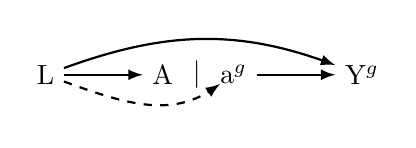
\begin{tikzpicture}[
array/.style={
    rectangle split,
	rectangle split parts = 3,
	rectangle split horizontal,
    minimum height = 2em
    }
]

\node (1) {L};
\node [array, right = of 1] (2) {
    {A}
    \nodepart{two}{$|$}
    \nodepart{three}{a$^g$}
};
\node [right = of 2] (3) {Y$^g$};

\draw[Arrow, thick] (1.east) -- (2.west);
\draw[Arrow, dashed] (1) to [out=340, in=215] (2.three);
\draw[Arrow, thick] (1) to [out=20, in=160] (3);

\draw[Arrow, thick] (2.east) -- (3.west);

\end{tikzpicture}
\caption{A SWIG representing a dynamic treatment regime.}
\label{fig:swig_det_dyn_inv}
\end{figure}

The joint density is:

\begin{equation}
    f(y,l,a,a^g) = f(y|l,a^g) f(a^g|l) f(a|l) f(l).
\end{equation}

After intervening on the exposure $A$, we have:

\begin{equation}
    f^G(y,l,a^g) = f(y|l,\textcolor{red}{a^g}) f(\textcolor{red}{a^g}|l) f(l).
\end{equation}

Thus, the expected value of the outcome $Y$ is:

\begin{align}
    \mathbb{E}^G \left[ Y \right] &= \sum_y y f^G(y) \\
    &= \sum_y y \sum_l \sum_{a^g} f^G(y,l,\textcolor{red}{a^g}) \\
    &= \sum_y \sum_l \sum_{a^g} y f(y|l,\textcolor{red}{a^g}) f(\textcolor{red}{a^g}|l) f(l) \\
    &= \sum_l \sum_{a^g} \mathbb{E} \left[ Y|A=\textcolor{red}{a^g},L=l\right] f(\textcolor{red}{a^g}|L=l) f(L=l).
\end{align}

\subsubsection{Deterministic Natural Treatment Regimes}
The rule for assigning treatment depends on its natural value.

\begin{figure}[ht]
\centering
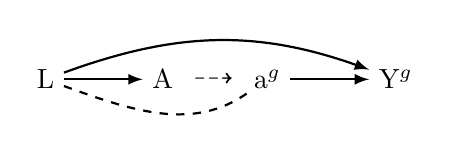
\begin{tikzpicture}[
array/.style={
    rectangle split,
	rectangle split parts = 3,
	rectangle split horizontal,
    minimum height = 2em
    }
]

\node (1) {L};
\node [array, right = of 1] (2) {
    {A}
    \nodepart{two}{$\dashrightarrow$}
    \nodepart{three}{a$^g$}
};
\node [right = of 2] (3) {Y$^g$};

\draw[Arrow, thick] (1.east) -- (2.west);
\draw[Arrow, dashed] (1) to [out=340, in=215] (2.three);
\draw[Arrow, thick] (1) to [out=20, in=160] (3);

\draw[Arrow, thick] (2.east) -- (3.west);

\end{tikzpicture}
\caption{A SWIG representing a natural treatment regime.}
\label{fig:swig_det_nat_inv}
\end{figure}

The joint density is:

\begin{equation}
    f(y,l,a,a^g) = f(y|l,a^g) f(a^g|l,a) f(a|l) f(l).
\end{equation}

After intervening on the exposure $A$, we have:

\begin{equation}
    f^G(y,l,a,a^g) = f(y|l,\textcolor{red}{a^g}) f(\textcolor{red}{a^g}|l,a) f(a|l) f(l).
\end{equation}

Thus, the expected value of the outcome $Y$ is:

\begin{align}
    \mathbb{E}^G \left[ Y \right] &= \sum_y y f^G(y) \\
    &= \sum_y y \sum_l \sum_a \sum_{a^g} f^G(y,l,a,\textcolor{red}{a^g}) \\
    &= \sum_y \sum_l \sum_a \sum_{a^g} y f(y|l,\textcolor{red}{a^g}) f(\textcolor{red}{a^g}|l,a) f(a|l) f(l) \\
    &= \sum_l \sum_a \sum_{a^g} \mathbb{E} \left[ Y|A=\textcolor{red}{a^g},L=l\right] f(\textcolor{red}{a^g}|a,L=l) f(a|l) f(L=l).
\end{align}

\subsubsection{Modified Treatment Policies}

\subsection{Random Treatment Regimes}
The rule for assigning treatment does so with probability between 0 and 1.

%%%%%%%%%%%%%%%%%%%%%%%%%%%%%%%%
\section{Time-varying Exposures}
%%%%%%%%%%%%%%%%%%%%%%%%%%%%%%%%

\subsection{Deterministic Treatment Regimes}
The rule for assigning treatment does so with probability 1.

\subsubsection{Deterministic Static Treatment Regimes}
The rule for assigning treatment does not depend on past treatment or covariates.

If $f^{\text{int}} (a_k | \bar{a}_{k-1}, \bar{D}_k=0)$ is either 0 or 1 for each $\bar{a}_k$ and for $k = 0,\dots,K$. In particular, given the regime $g = (g_0,\dots,g_K)$, $f^{\text{int}} (a_k | \bar{a}_{k-1}^g, \bar{D}_k=0) = 1$ if $a_k = a_k^g$, and 0 otherwise, with $a_s^g = g_s(\bar{a}_{s-1}^g)$.

\begin{figure}[ht]
\centering
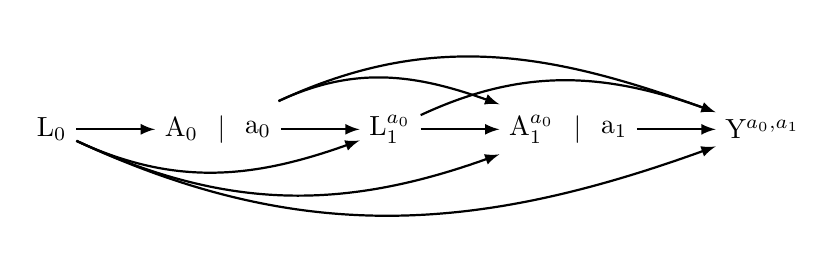
\begin{tikzpicture}[
array/.style={
    rectangle split,
	rectangle split parts = 3,
	rectangle split horizontal,
    minimum height = 2em
    }
]

\node (1) {L$_0$};
\node [array, right = of 1] (2) {
    {A$_0$}
    \nodepart{two}{$|$}
    \nodepart{three}{a$_0$}
};
\node [right = of 2] (3) {L$_1^{a_{0}}$};
\node [array, right = of 3] (4) {
 	{A$_1^{a_{0}}$}
    \nodepart{two}{$|$}
    \nodepart{three}{a$_1$}
};
\node [right = of 4] (5) {Y$^{a_0, a_1}$};

\draw[Arrow, thick] (1.east) -- (2.west);
\draw[Arrow, thick] (1) to [out=335, in=200] (3);
\draw[Arrow, thick] (1) to [out=335, in=200] (4);
\draw[Arrow, thick] (1) to [out=335, in=200] (5);

\draw[Arrow, thick] (2.east) -- (3.west);
\draw[Arrow, thick] (2) to [out=25, in=160] (4);
\draw[Arrow, thick] (2) to [out=25, in=160] (5);

\draw[Arrow, thick] (3.east) -- (4.west);
\draw[Arrow, thick] (3) to [out=25, in=160] (5);

\draw[Arrow, thick] (4.east) -- (5.west);

\end{tikzpicture}
\caption{A SWIG representing a static treatment regime.}
\label{fig:swig_det_stat}
\end{figure}

The joint density is:

\begin{align}
    f(y,l_0,l_1,a_0,a_1) = &f(y|l_0,l_1,a_0,a_1)\times\\
    &f(a_1|l_0,l_1,a_0) \times f(l_1|l_0,a_0)\times\\
    &f(a_0|l_0) \times f(l_0).
\end{align}

After intervening on the exposure $A$ at both time points, we have:

\begin{align}
    f^G(y,l_0,l_1,a_0,a_1) = &f(y|l_0,l_1,\textcolor{red}{a_0},\textcolor{red}{a_1})\times\\
    &f(\textcolor{red}{a_1}|l_0,l_1,\textcolor{red}{a_0}) \times f(l_1|l_0,\textcolor{red}{a_0})\times\\
    &f(\textcolor{red}{a_0}|l_0) \times f(l_0).
\end{align}

Thus, the expected value of the outcome $Y$ is:

\begin{align}
    \mathbb{E}^G \left[ Y \right] &= \sum_y y f^G(y) \\
    &= \sum_y y \sum_{l_0} \sum_{l_1} \sum_{a_0} \sum_{a_1} f^G(y,l_0,l_1,\textcolor{red}{a_0},\textcolor{red}{a_1}) \\
    &= \sum_{l_0} \sum_{l_1} \sum_{a_0} \sum_{a_1}
    \!\begin{aligned}[t] \label{eq:gform_long_static}
        &\mathbb{E} \left[ Y|L_0=l_0,L_1=l_1,A_0=\textcolor{red}{a_0},A_1=\textcolor{red}{a_1} \right]\times\\
        &f(\textcolor{red}{a_1}|l_0,l_1,\textcolor{red}{a_0})\times\\
        &f(l_1|l_0,\textcolor{red}{a_0})\times\\
        &f(\textcolor{red}{a_0}|l_0)\times\\
        &f(l_0).
    \end{aligned}
\end{align}

\paragraph*{Algorithms}
One estimator of $\mathbb{E}^G [Y]$ is the \textbf{parametric g-computation formula}. For the case of a deterministic static intervention with one exposure and two time points, we can rewrite Equation \ref{eq:gform_long_static} so that it corresponds to a series of conditional expectations:

\begin{align}
    \mathbb{E}^G \left[ Y \right]
    &= \sum_{l_0} \sum_{l_1} \sum_{a_0} \sum_{a_1}
    \!\begin{aligned}[t]
        &\mathbb{E} \left[ Y|L_0=l_0,L_1=l_1,A_0=\textcolor{red}{a_0},A_1=\textcolor{red}{a_1} \right] \times \\
        &f(\textcolor{red}{a_1}|l_0,l_1,\textcolor{red}{a_0}) \times f(l_1|l_0,\textcolor{red}{a_0}) \times \\
        &f(\textcolor{red}{a_0}|l_0) \times f(l_0)
    \end{aligned} \\
    &= \sum_{l_0} \sum_{l_1} \sum_{a_0} \sum_{a_1}
    \!\begin{aligned}[t] \label{eq:nested_gcom_long_static}
        &\mathbb{E} \left[ Y|L_0=l_0,L_1=l_1,A_0=\textcolor{red}{a_0},A_1=\textcolor{red}{a_1} \right] \times \\
        &f(\textcolor{red}{a_1},l_1|l_0,\textcolor{red}{a_0}) \times \\
        &f(\textcolor{red}{a_0},l_0).
    \end{aligned}
\end{align}

Equation \ref{eq:nested_gcom_long_static} suggests a different form for the parametric g-computation formula, which in the literature is usually called iterated conditional expectation (ICE) g-computation formula. The pseudo-algorithm then reads as follows ($\bar{A}_t$ means the history of $A$ up to time $t$):

\begin{enumerate}
    \item Fit a regression model with dependent variable $Y$ and independent variables $\bar{A}$ and $\bar{L}$.
    \item 
    \item Estimate the outcome $Y^a$ using the model fit in the previous point but changing the exposure according to the intervention rule $G$.
    \item Take the average of $\hat{Y}^a$ over the confounders $L$.
\end{enumerate}

In the case of multiple exposures (e.g., if $A$ is actually a vector of variables), the g-formula would remain the same \footnote{We are assuming that there would be \textbf{no arrow} between exposure nodes in the SWIG, that is: $f(a_1,a_2|l) = f(a_1|l) \times f(a_2|l)$. This means that the correlation between them is due to e.g., a common source, but the exposures themselves are not causally related.}, but the pseudo-algorithm should be modified to take into account that the intervention rule now applies to all exposures $a \in \mathbf{A}$.

\subsubsection{Deterministic Dynamic Treatment Regimes}
The rule for assigning treatment depends on past treatment or covariates.

If $f^{\text{int}} (a_k | \bar{l}_k, \bar{a}_{k-1}, \bar{D}_k=0)$ is either 0 or 1 for each $(\bar{a}_k, \bar{l}_k)$ and for $k = 0,\dots,K$. In particular, given the regime $g = (g_0,\dots,g_K)$, $f^{\text{int}} (a_k | \bar{l}_k, \bar{a}_{k-1}^g, \bar{D}_k=0) = 1$ if $a_k = a_k^g$, and 0 otherwise, with $a_s^g = g_s(\bar{l}_s, \bar{a}_{s-1}^g)$.

\subsubsection{Deterministic Natural Treatment Regimes}
The rule for assigning treatment depends on its natural value.

\begin{figure}[ht]
\centering
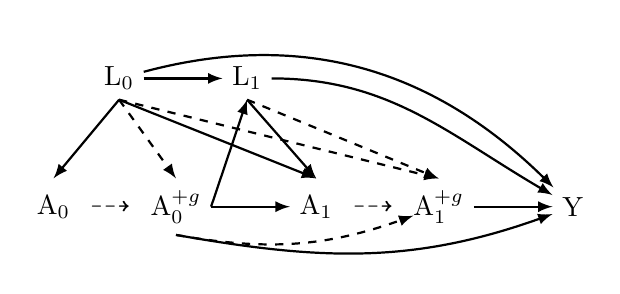
\begin{tikzpicture}[
array/.style={
    rectangle split,
	rectangle split parts = 3,
	rectangle split horizontal,
    minimum height = 2em
    }
]

\node (1) {L$_0$};
\node [array, below = of 1] (2) {
    {A$_0$}
    \nodepart{two}{$\dashrightarrow$}
    \nodepart{three}{A$_0^{+g}$}
};
\node [right = of 1] (3) {L$_1$};
\node [array, right = of 2] (4) {
 	{A$_1$}
    \nodepart{two}{$\dashrightarrow$}
    \nodepart{three}{A$_1^{+g}$}
};
\node [right = of 4] (5) {Y};

\draw[Arrow, thick] (1.south) -- (2.one north);
\draw[Arrow, dashed] (1.south) -- (2.three north);
\draw[Arrow, thick] (1.east) -- (3.west);
\draw[Arrow, thick] (1) to [out=15, in=135] (5);
\draw[Arrow, thick] (1.south) -- (4.one north);
\draw[Arrow, dashed] (1.south) -- (4.three north);

\draw[Arrow, thick] (2.three east) -- (3.south);
\draw[Arrow, thick] (2.three east) -- (4.one west);
\draw[Arrow, thick] (2.three south) to [out=350, in=200] (5);
\draw[Arrow, dashed] (2.three south) to [out=350, in=200] (4.three);

\draw[Arrow, thick] (3.south) -- (4.one north);
\draw[Arrow, dashed] (3.south) -- (4.three north);
\draw[Arrow, thick] (3.east) to [out=360, in=150] (5);

\draw[Arrow, thick] (4.east) -- (5.west);

\end{tikzpicture}
\caption{A SWIG representing a natural treatment regime.}
\label{fig:swig_det_nat}
\end{figure}

The joint density is:

\begin{align}
    f(y,l_0,l_1,a_0,a_0^g,a_1,a_1^g) = &f(y|l_0,l_1,a_0^g,a_1^g)\times\\
    &f(a_1^g|l_0,l_1,a_0^g,a_1)\times\\
    &f(a_1|l_0,l_1,a_0^g)\times\\
    &f(l_1|l_0,a_0^g)\times\\
    &f(a_0^g|l_0,a_0)\times\\
    &f(a_0|l_0) f(l_0).
\end{align}

After intervening on the exposure $A$, we have:

\begin{align}
    f^G(y,l_0,l_1,a_0,a_0^g,a_1,a_1^g) = &f(y|l_0,l_1,\textcolor{red}{a_0^g},\textcolor{red}{a_1^g)}\times\\
    &f(\textcolor{red}{a_1^g}|l_0,l_1,\textcolor{red}{a_0^g},a_1)\times\\
    &f(a_1|l_0,l_1,\textcolor{red}{a_0^g})\times\\
    &f(l_1|l_0,\textcolor{red}{a_0^g})\times\\
    &f(\textcolor{red}{a_0^g}|l_0,a_0)\times\\
    &f(a_0|l_0) f(l_0).
\end{align}

Thus, the expected value of the outcome $Y$ is:

\begin{align}
    \mathbb{E}^G \left[ Y \right] &= \sum_y y f^G(y) \\
    &= \sum_y y \sum_{l_0} \sum_{l_1} \sum_{a_0} \sum_{a_0^g} \sum_{a_1} \sum_{a_1^g} f^G(y,l_0,l_1,a_0,\textcolor{red}{a_0^g},a_1,\textcolor{red}{a_1^g}) \\
    &= \sum_{l_0} \sum_{l_1} \sum_{a_0} \sum_{a_0^g} \sum_{a_1} \sum_{a_1^g}
    \!\begin{aligned}[t]
        &\mathbb{E} \left[ Y|L_0=l_0,L_1=l_1,A_0=\textcolor{red}{a_0^g},A_1=\textcolor{red}{a_1^g} \right]\times\\
        &f(\textcolor{red}{a_1^g}|l_0,l_1,\textcolor{red}{a_0^g},a_1)\times\\
        &f(a_1|l_0,l_1,\textcolor{red}{a_0^g})\times\\
        &f(l_1|l_0,\textcolor{red}{a_0^g})\times\\
        &f(\textcolor{red}{a_0^g}|l_0,a_0)\times\\
        &f(a_0|l_0) f(l_0).
    \end{aligned}
\end{align}

\subsubsection{Modified Treatment Policies}

\subsection{Random Treatment Regimes}
The rule for assigning treatment does so with probability between 0 and 1.

\subsubsection{Random Static Treatment Regimes}
The rule for assigning treatment does not depend on past covariates.

\subsubsection{Random Dynamic Treatment Regimes}
The rule for assigning treatment depends on past covariates.

\subsubsection{Random Natural Treatment Regimes}
The rule for assigning treatment depends on its natural value.

\subsubsection{Modified Treatment Policies}

\end{document}
